\documentclass[serif, aspectratio=169]{beamer}
%\documentclass[serif]{beamer}  % for 4:3 ratio

\RequirePackage{minted2}
\usepackage[T1]{fontenc} 
\usepackage[utf8]{inputenc}
\usepackage{fourier} % see "http://faq.ktug.org/wiki/uploads/MathFonts.pdf" for other options
\usepackage{hyperref}
\usepackage{latexsym,amsmath,xcolor,multicol,booktabs,calligra}
\usepackage{graphicx,pstricks,listings,stackengine}
\usepackage{lipsum}
\usepackage{../HKUSTstyle}

%imports customs%
\usepackage{caption}    % for subfigures
\usepackage{subcaption} % for subfigures
\usepackage{ragged2e}
\usepackage{booktabs,makecell}
\usepackage{colortbl}
\usepackage{multirow}
\usepackage{cite}
\usepackage{tcolorbox}
\usepackage[sort,authoryear]{natbib}

\author{Julien Bezançon}

\title{Python Programmation}
\subtitle{CM 4~: Functional Programming}

\institute{julien.bezancon@univ-lorraine.fr / \url{https://julienbez.github.io}}

\date{}

% defs
\def\cmd#1{\texttt{\color{red}\footnotesize $\backslash$#1}}
\def\env#1{\texttt{\color{blue}\footnotesize #1}}

% set colors
\definecolor{hkustyellow}{RGB}{167, 131, 55}
\definecolor{hkustblue}{RGB}{0, 56, 116}
\definecolor{hkustred}{RGB}{209, 51, 59}

\lstset{
    basicstyle=\ttfamily\small,
    keywordstyle=\bfseries\color{deepblue},
    emphstyle=\ttfamily\color{deepred},    % Custom highlighting style
    stringstyle=\color{deepgreen},
    numbers=left,
    numberstyle=\small\color{halfgray},
    rulesepcolor=\color{red!20!green!20!blue!20},
    frame=shadowbox,
}

\begin{document} %  --- --- --- --- --- --- --- --- --- --- --- --- 

\begin{frame}[noframenumbering,plain]
    \titlepage
    \vspace*{-0.6cm}
    \begin{figure}[htpb]
        \begin{center}
            \hspace{0.3cm}
            
\includegraphics[width=0.7\columnwidth]{../../../IMAGES/loria_idmc.png}
        \end{center}
    \end{figure}
\end{frame}

% \begin{frame}    
%     \tableofcontents[sectionstyle=show,
%     subsectionstyle=show/shaded/hide,
%     subsubsectionstyle=show/shaded/hide]
% \end{frame}

\section{Before we start...}

\begin{exoframe}
    \begin{center}
        \Large
        What did you learn during last lecture ? \\
        Any questions ?
    \end{center}
\end{exoframe}

\begin{frame}{Last Lecture Doggy bag}
    \begin{minipage}{0.45\columnwidth}
        \begin{block}{Functions}
            \begin{itemize}
                \item Function definition and calling
                \item Parameters and arguments
                \item Variadic arguments
                \item Python scopes
            \end{itemize}
        \end{block}
        \begin{block}{Advanced strings}
            \begin{itemize}
                \item Special characters handling
                \item String formatting
                % \item Range
            \end{itemize}
        \end{block}
    \end{minipage}
    \hfill
    \begin{minipage}{0.45\columnwidth}
        \begin{figure}
            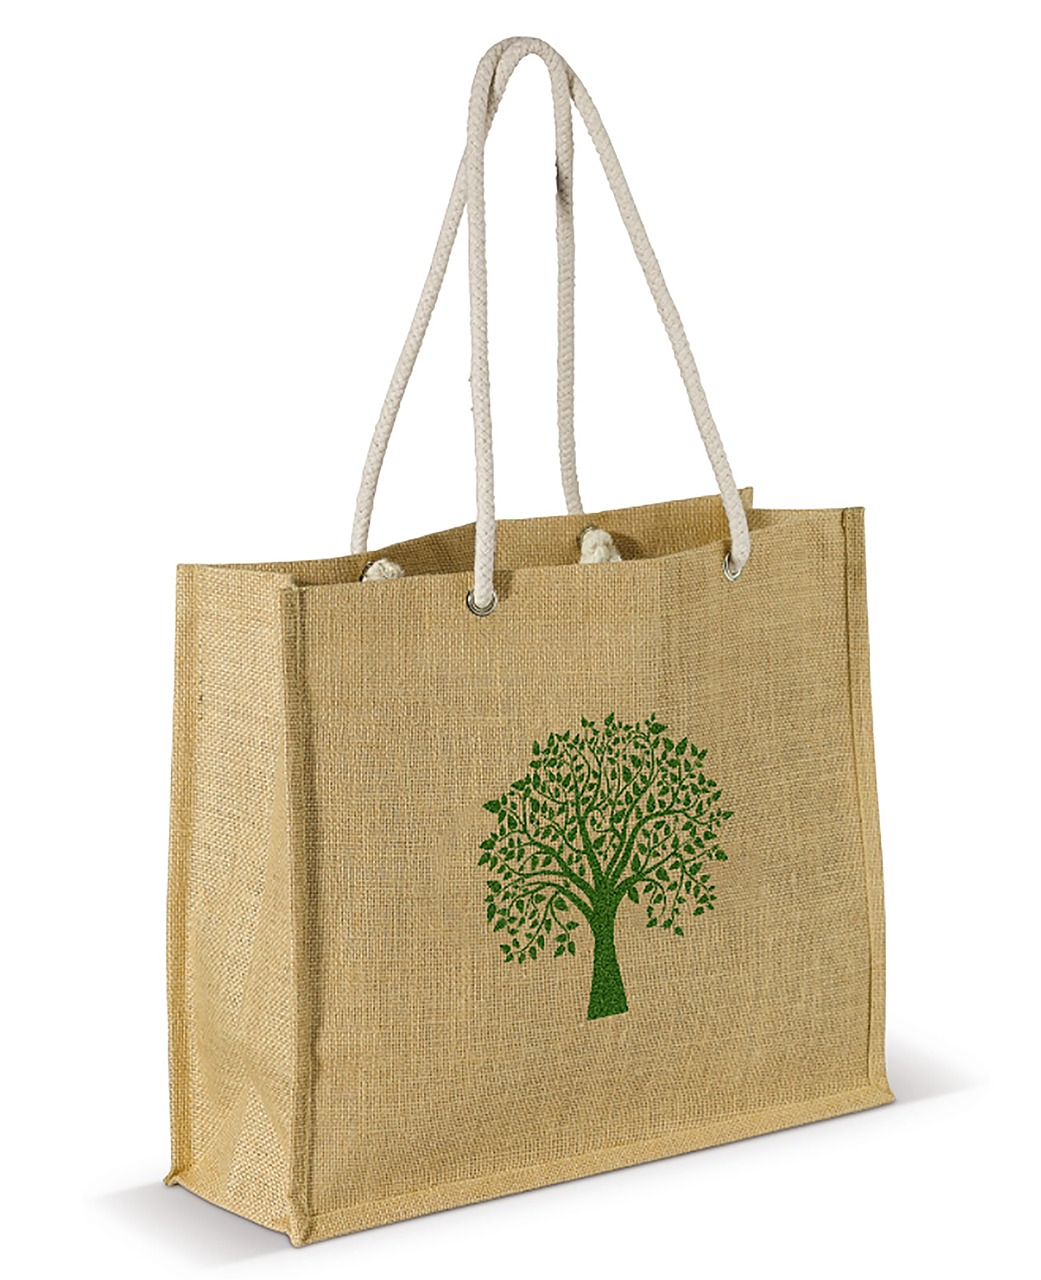
\includegraphics[width=0.9\columnwidth]{../../../FIGURES/divers/doggybag.jpg}
        \end{figure}
    \end{minipage}
\end{frame}

\section{Programming Paradigms}

% procedural, declarative, oo et functional
% montrer des exemples à chaque fois
% slide résumant ce que c'est que le functional

% voir partie 1 du CM functional programming de tom



\end{document}
